\documentclass{ximera}

\input{../../preamble.tex}

\title{Linear Transformation Cartoons}

\begin{document}
\begin{abstract}
We draw pictures representing linear transformations.
\end{abstract}
\maketitle

We will call the pictures we draw representing linear transformations ``cartoons,'' not because they are humorous, but because they will only expose a portion of the truth.  A Bugs Bunny cartoon might give us some insights on human nature, but the rules of physics and biology are routinely (and grossly) violated.  So it will be with our \dfn{linear transformation cartoons}.  Here is our first, followed by a guide to help you understand how these are meant to describe fundamental truths about linear transformations, while simultaneously violating other truths.

\begin{image}
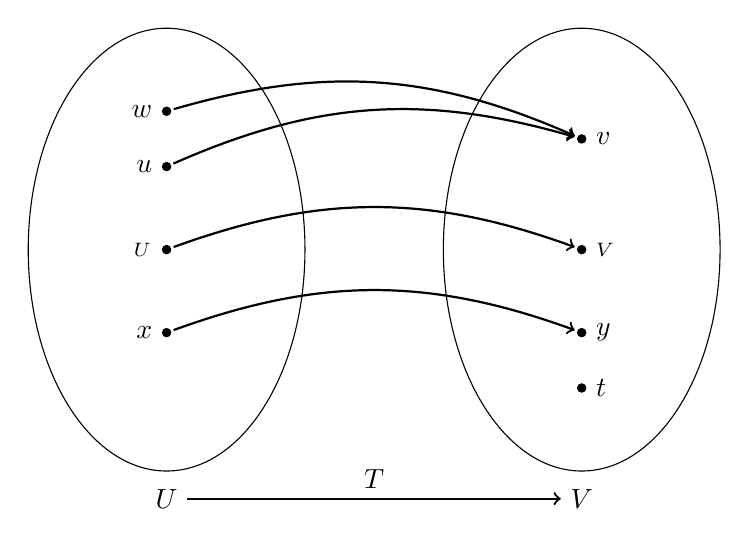
\begin{tikzpicture}
\tikzset{ltvect/.style={shape=circle, minimum size=0.30em, inner sep=0pt, draw, fill=black}}
\tikzset{ltedge/.style={->, bend left=20, thick, shorten <=0.1em, shorten >=0.1em}}
<!--  base generic picture, equal ovals -->
<!--  vertical axes at x = 5, x = 20  space is [x=10 to x=15] -->
\draw ( 5em, 8em) circle [x radius=5em, y radius=8em, thick];
\draw (20em, 8em) circle [x radius=5em, y radius=8em, thick];
\node (U) at ( 5em, -1em) {$U$};
\node (V) at (20em, -1em) {$V$};
\draw[->, thick, draw] (U) to node[auto] {$T$} (V);
<!--  inputs -->
\node (w)     [ltvect, label=left:$\vect{w}$]      at (5em, 13em) {};
\node (u)     [ltvect, label=left:$\vect{u}$]      at (5em, 11em) {};
\node (zeroU) [ltvect, label=left:$\zerovector_U$] at (5em,  8em) {};
\node (x)     [ltvect, label=left:$\vect{x}$]      at (5em,  5em) {};
<!--  outputs -->
\node (v)     [ltvect, label=right:$\vect{v}$]      at (20em, 12em) {};
\node (zeroV) [ltvect, label=right:$\zerovector_V$] at (20em,  8em) {};
\node (y)     [ltvect, label=right:$\vect{y}$]      at (20em,  5em) {};
\node (t)     [ltvect, label=right:$\vect{t}$]      at (20em,  3em) {};
<!--  associations -->
\draw[ltedge] (u)     to (v);
\draw[ltedge] (w)     to (v);
\draw[ltedge] (zeroU) to (zeroV);
\draw[ltedge] (x)     to (y);
\end{tikzpicture}
\end{image}

Here we picture a linear transformation $\ltdefn{T}{U}{V}$, where this
information will be consistently displayed along the bottom edge.  The
ovals are meant to represent the vector spaces, in this case $U$, the
domain, on the left and $V$, the codomain, on the right.  Of course,
vector spaces are typically infinite sets, so you will have to imagine
that characteristic of these sets.  A small dot inside of an oval will
represent a vector within that vector space, sometimes with a name,
sometimes not (in this case every vector has a name).  The sizes of
the ovals are meant to be proportional to the dimensions of the vector
spaces.  However, when we make no assumptions about the dimensions, we
will draw the ovals as the same size, as we have done here (which is
not meant to suggest that the dimensions have to be equal).

To convey that the linear transformation associates a certain input
with a certain output, we will draw an arrow from the input to the
output.  So, for example, in this cartoon we suggest that
$\lteval{T}{\vect{x}}=\vect{y}$.  Nothing in the definition of a linear
transformation prevents two different inputs being sent to the same
output and we see this in
$\lteval{T}{\vect{u}}=\vect{v}=\lteval{T}{\vect{w}}$.  Similarly, an output
may not have any input being sent its way, as illustrated by no arrow
pointing at $\vect{t}$.  In this cartoon, we have captured the essence
of our one general theorem about linear transformations,
\ref{theorem:LTTZZ}, $\lteval{T}{\zerovector_U}=\zerovector_V$.  On
occasion we might include this basic fact when it is relevant, at
other times maybe not.  Note that the definition of a linear
transformation requires that it be a function, so every element of the
domain should be associated with some element of the codomain.  This
will be reflected by never having an element of the domain without an
arrow originating there.

These cartoons are of course no substitute for careful definitions and
proofs, but they can be a handy way to think about the various
properties we will be studying.

\end{document}

%%% Local Variables:
%%% mode: latex
%%% TeX-master: t
%%% End:
